In this section, we describe our methodology for preparing the data to answer our research questions.

The aim of this paper is to understand how logs are changed during bug fixes and the relationship between bug resolution time and log changes. We conduct a case study on three open source platform software projects, i.e., \textsl{Hadoop, HBase} and \textsl{Qpid}. All three platform softwares projects have extensive logging in their source code. Table~\ref{tba:Overview} highlights the overview of the three platform software projects.

\begin{table}[t]
	\protect\caption{An overview of the platform software projects}
	\label{tba:Overview}
	\centering{}%
	\begin{tabular}{|>{\centering}p{.15\textwidth}|>{\centering}p{.1\textwidth}|>{\centering}p{.1\textwidth}|>{\centering}p{.1\textwidth}|>{\centering}p{.1\textwidth}|>{\centering}p{.1\textwidth}|>{\centering}p{.1\textwidth}|}
		\hline 
		\multirow{2}{*}{Projects} & \multicolumn{2}{c|}{Hadoop} & \multicolumn{2}{c|}{HBase} & \multicolumn{2}{c|}{Qpid}\tabularnewline
		\cline{2-7} 
		& Bug fixing  & Non-bug fixing & Bug fixing  & Non-bug fixing & Bug fixing  & Non-bug fixing \tabularnewline
		\hline 
		Total \# of commits & 1,808 & 1,809 & 1924 & 1463 & 953 & 875\tabularnewline
		
		
		 & (49.9 \%) & (50.1 \%) & (56.8 \%) & (43.2 \%) & (52.1 \%) & (47.9 \%) \tabularnewline
		\hline 
		 
		Code churn (SLOC) & 246 K & 1.8 M & 653 K & 1.5 M &  106 k & 597 K\tabularnewline
		\hline 
		Log churn  & 3,536 & 16,980 & 4,672 & 10,335 & 972 & 4,953\tabularnewline
		\hline 
		\% of Commits with log churn & 24.0 \% (433) &  46.2 \% (656) & 36.2 \% (648) & 42.1 \% (616) & 22.1 \% (211) & 32.8 \% (287) \tabularnewline
		\hline		
	\end{tabular}
\end{table}



{\textbf{Hadoop}\footnote[1]{http://hadoop.apache.org/}}: \emph{Hadoop} is an open source platform for distributed storage and processing of big data on computer clusters. \emph{Hadoop} uses the MapReduce data-processing paradigm. The logging characteristics of \emph{Hadoop} have been extensively studied in prior research~\cite{JGLouMining,EMSEIAN,ConsoleLogs}. We study the changes to logs from \emph{Hadoop} releases $0.16.0$ to $2.0$.


{\textbf{HBase}\footnote[2]{http://hbase.apache.org/}}: \emph{HBase} is a distributed, scalable, big data software, which uses \emph{Hadoop} file-systems. We study the changes to logs in \emph{HBase} from release $0.10$ to $0.98.2.RC0$. This covers more than four years of development in \emph{HBase} from 2010 to 2014.

{\textbf{Qpid}\footnote[3]{https://qpid.apache.org}}: \emph{Qpid} is an open source messaging platform that implements an Advanced Message Queuing Protocol (AMQP). We study \emph{Qpid} release $0.10$ to release $0.30$ that are from 2011 till 2014.


Figure~\ref{tba:Overview} shows a general overview of our approach, which consists of four steps: (1) We mine the git repository of each studied system to extract all commits, and identify bug-fixing commits (bug fixes) non-bug-fixing commits (non-bug fixes). (2) We identify log changes in both bug fixes and non-bug fixes. (3) We categorize the log changes into three types, \textsl{`New logs', `Modified Logs'} and \textsl{`Deleted logs'}. (4) We calculate churn metrics for each type and use a statistical tool R~\cite{ihaka1996r}, to perform experiments on the data to answer our research questions.  In the reminder of this section we describe the first three steps.

%We used Apache software versioning system, SVN to collect the commit
%history for all the projects in our case study. We used JIRA to collect
%the buggy reports for all the projects in our case study. We extracted
%the reports in XML format for parsing convenience. 


\subsection{Study Approach}

In this section, we present the first three steps of our study approach. 
%We use Git to study the evolution of Java source code in the three subject systems. 
%%similar to C-REX ~\cite{HassanPHD} and J-REX ~\cite{WCSEIan}. 
%We extract the changes in each commit and use this data to calculate the metrics to answer our research questions.
\begin{figure}[t]
	\centering
	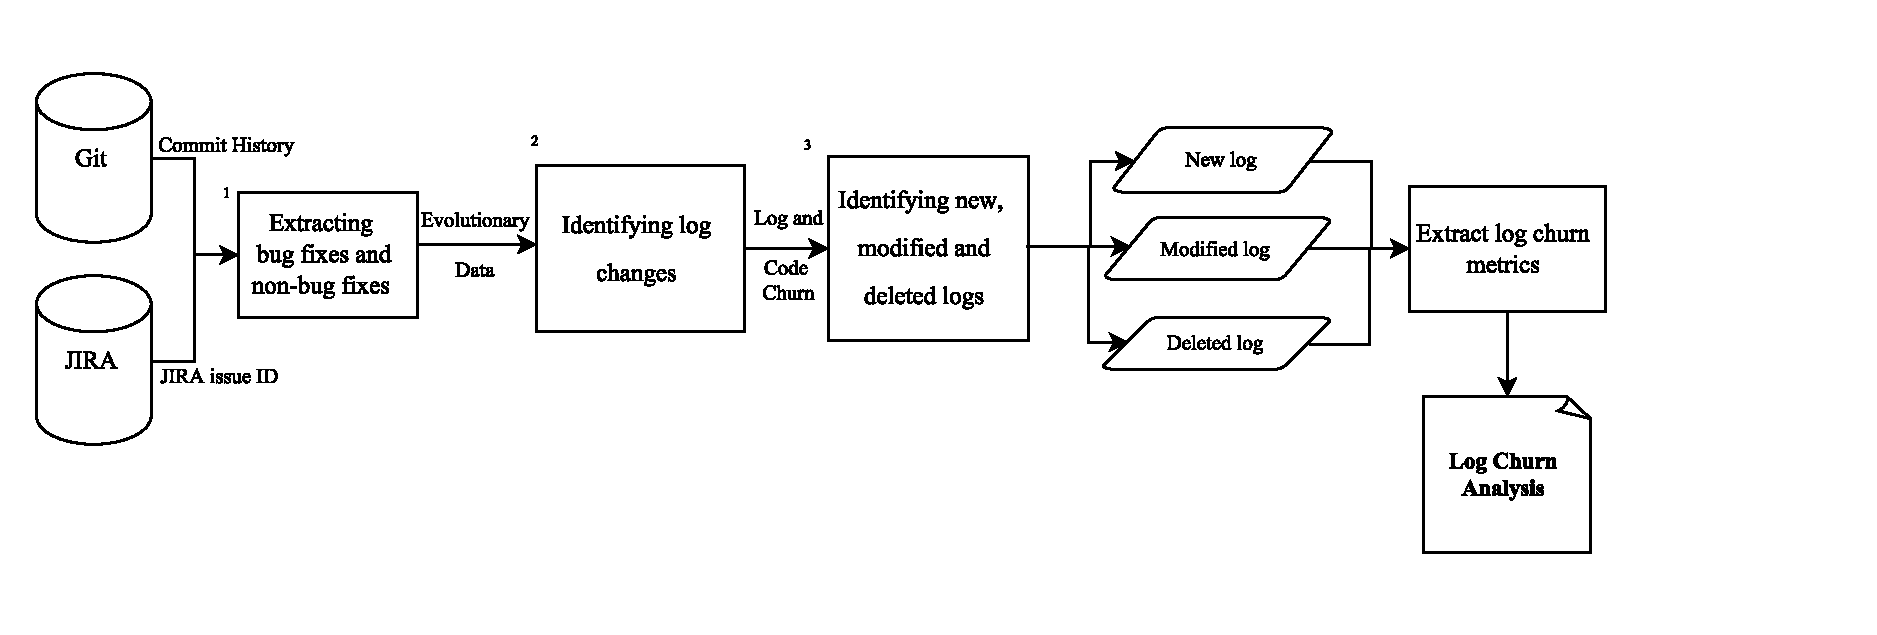
\includegraphics[scale=0.45]{MethdologyICESEM}
	\caption{Overview of our case study approach }
	\label{fig:MethodologyICSME}
\end{figure}

\subsubsection{Extracting bug fixes and non-bug fixes}

The first step in our approach is to extract commits that are associated with bug fixes and the ones that are not associated with bug fixes. First, we extract a list of all commits from the git repository of each project. To avoid the branching and merging commits, we enable the `no-merges' option in the git \textsl{log} command. This flattens all the changes that are made to file in different branches and excludes the final merge between branch and trunk. We also filter out the changes to non-Java files or the test files from the commits. 

Next, we extract a list of all the JIRA issues that have the type \emph{bug}. Developers often mention the JIRA issue ID's in the commit messages. We search JIRA issue IDs in the commit messages to identify all the bug fixes. We exclude commits that do not contain any JIRA ID since we cannot identify if the commit is a bug fix or not. 

\subsubsection{Identifying log changes}

To identify the log changes in the datasets, we first manually explore logs in the source code. Some logs are specific to a particular project. For example, a log from Qpid invokes `QPID\_LOG' to print logs as follows: 
\hypobox{QPID\_LOG(error, ``Rdma: Cannot accept new connection (Rdma exception):
	'' + e.what());
	}

Some logs leverage logging libraries to print logs. For example, \textsl{Log4j}\footnote{http://logging.apache.org/log4j/1.2/} is used widely in \emph{Hadoop} and \emph{HBase}. In both projects, logs have a method invocation `LOG', followed by a logging level. The following log uses \textsl{Log4j}:
\hypobox{ LOG.debug(``public AsymptoticTestCase(String''+ name +``) called'')}

Using regular expressions to match these logs, we automate the process of finding all the logs in the studied projects.


\subsubsection{Identifying new, modified and deleted logs}

Since git \textsl{diff} does not track modification to the code, modifications to a log is shown as a deletion followed by an addition. To track these added and deleted logs we used Levenshtein ratio~\cite{Levenshtein2}. For every pair of added or deleted logs in a commit, we compare the text in parenthesis after removing the logging method (e.g, LOG ) and the log level (e.g, info). We calculate the Levenshtein ratio between the added and deleted log similar to prior research~\cite{levenshteinratio}. We consider a pair of added and deleted logs as a log modification if they have a Levenshtein ratio of 0.6 or higher. For example, the logs shown below have Levenshtein ratio of 0.86. Hence such a pair of added and deleted logs are categorized as a log modification.  
\hypobox{+      LOG.debug(``Call: " +method.getName()+`` took "+ callTime + ``ms");\\ 
	-        LOG.debug(``Call: " +method.getName()+ `` " + callTime);} 

If an added log has a Levenshtein ratio higher than 0.6 with more than one deleted log, we consider the pair of added and deleted logs with the highest Levenshtein ratio as a log modification. After identifying all log modifications, we identify three types of log changes in a commit namely `new logs', `deleted logs' and `modified logs'.

